\documentclass[10pt,a4paper,titlepage,oneside]{article}
\usepackage[utf8]{inputenc}
\usepackage[german]{babel}
\usepackage{amsmath}
\usepackage{amsfonts}
\usepackage{amssymb}
\usepackage[left=2cm,right=2cm,top=2cm,bottom=2cm]{geometry}
\usepackage{graphicx}
\usepackage[hidelinks]{hyperref}

%Die folgenden drei Befehle sorgen für Rahmen um die Bilder herum.
%\usepackage{float}\floatstyle{boxed}\restylefloat{figure}

\author{Dr. Martin Mandelkow}
\title{Handbuch Apotheken-Dienstplan}










\begin{document}
\maketitle
\tableofcontents\pagebreak










\section{Copyright}
Die Software ist bis auf Weiteres vollständiges Eigentum von Dr. Martin Mandelkow.
Eventuell wird in der Zukunft eine Version unter einer GPL Lizenz veröffentlicht werden.










\section{Einführung}
Das Ziel dieser Software ist es - mit möglichst wenig Aufwand, Fehlern und Zeit - Dienstpläne zu gestalten, die für Mitarbeiter, Patienten und die Apothekenkeitung optimal sind.

Dabei werden Aufwand im Abverkauf, stetige Anwesenheit von Approbierten und Abwesenheitszeiten (z.B. Urlaub, Krankheit) berücksichtigt. Mittagspausen werden explizit vorgegeben.

Es ist vorgesehen, dass es einen Grundplan gibt, nach dem alle Mitarbeiter eingesetzt werden. Dieser soll die persönlichen Wünsche der Mitarbeiter berücksichtigen.
%Dazu gibt es einen Wunschplan. Dieser ist Interessant für Abweichungen vom üblichen Plan bei Urlaub und Abwesenheit.

Bisher existieren folgende Ansichten:
\begin{itemize}
	\item Tag
	\item Woche
	\item Personen
	\item Stunden
	\item Abwesenheit
\end{itemize}

Außer für die Personenansicht gibt es jeweils eine Bearbeitungs-Version.
Die Bearbeitungsversionen können und dürfen nur durch dafür bestimmte Mitarbeiter genutzt werden. Derzeit ist das ausschließlich Dr. Mandelkow.

\subsubsection{Technisches}
Das Programm basiert auf einer MYSQL-Datenbank und einem PHP-Frontend.
Es werden HTML5-Elemente und CSS genutzt.










\section{Kontakt und Unterstützung}
Ich stehe jederzeit gerne für Fragen zur Verfügung.
Außerhalb der regulären Arbeitszeit bin ich unter der Adresse \href{mailto:dienstplan@martin-mandelkow.de}{dienstplan@martin-mandelkow.de} zu erreichen.










\section{Benutzung des Dienstplanes}
\subsection{Ausgabe zum Lesen}
\subsubsection{Zugang}
Der Zugang zum Dienstplanprogramm erfolgt über die Domain martin-mandelkow.de unter der URL \url{https://martin-mandelkow.de/apotheke/dienstplan}.
Derzeit gibt es einen gemeinsamen Zugang für alle Mitarbeiter.
\begin{itemize}
	\item User Name: Mitarbeiter
	\item Password: GrosseFreude
\end{itemize}



\paragraph{Technisches}
\begin{sloppypar}Der Server kommuniziert ausschließlich verschlüsselt über das HTTPS Protokoll.
Die Zugangsverwaltung erfolgt derzeit über den Apache Server mittels htaccess.
Das Anlegen neuer Benutzer kann mit \mbox{\texttt{htpasswd -c /var/www/.htpasswd \emph{Benutzer}}}
erfolgen. Welche Benutzer welche Rechte haben, wird in der Datei \mbox{\texttt{/etc/httpd/conf/httpd.conf}} festgelegt:
\end{sloppypar}

\begin{verbatim}
<Directory /var/www/html/apotheke>
<Files *-in.php>
    AuthType basic
    AuthName "Nur fuer Administratoren"
    AuthUserFile /var/www/.htpasswd
    Require user Mandelkow Kreimann
</Files>
AuthBasicProvider file
AuthUserFile /var/www/.htpasswd
AuthGroupFile /dev/null
AuthName "Dieser Bereich ist passwortgeschuetzt fuer Mitarbeiter."
AuthType Basic
require valid-user
</Directory>
\end{verbatim}





\subsubsection{Tag}
Die Tagesansicht besteht aus einer Tabelle mit den Informationen,
\begin{itemize}
	\item VK-Nummer
	\item Nachname
	\item Dienstbeginn und Dienstende
	\item Mittagsbeginn und Mittagsende (wenn vorhanden)
\end{itemize}
und zwei Abbildungen. Die obere Abbildung zeigt die Informationen der Tabelle in Form eines Balkendiagrammes. Zusätzlich ist die Gesamtstundenzahl des Tages für jeden Mitarbeiter angegeben (Abb. \ref{fig:Tagesansicht}).

Im darunter liegenden Bild finden sich zwei Histogramme. In roter Farbe ist der erwartete Arbeitsaufwand im Verkauf dargestellt. Hierzu werden die Faktoren Monat, Tag im Monat, Wochentag und Uhrzeit berücksichtigt. Die Erfassung der Daten erfolgt aus der PEP-Exportfunktion der ASYS-Software. Derzeit muss eine solche Datei manuell über einen sicheren Transport (z.B. SFTP) zum Server transportiert werden.

Die Anzahl der vorhandenen Mitarbeiter wird durch die grüne Linie wiedergegeben. In der Darstellung wird durchgehend ein Mitarbeiter abgezogen. So ist für Ware, Telefon und sonstige Arbeiten im Backoffice immer eine Person vorgesehen.
\begin{figure}[h]
\centering
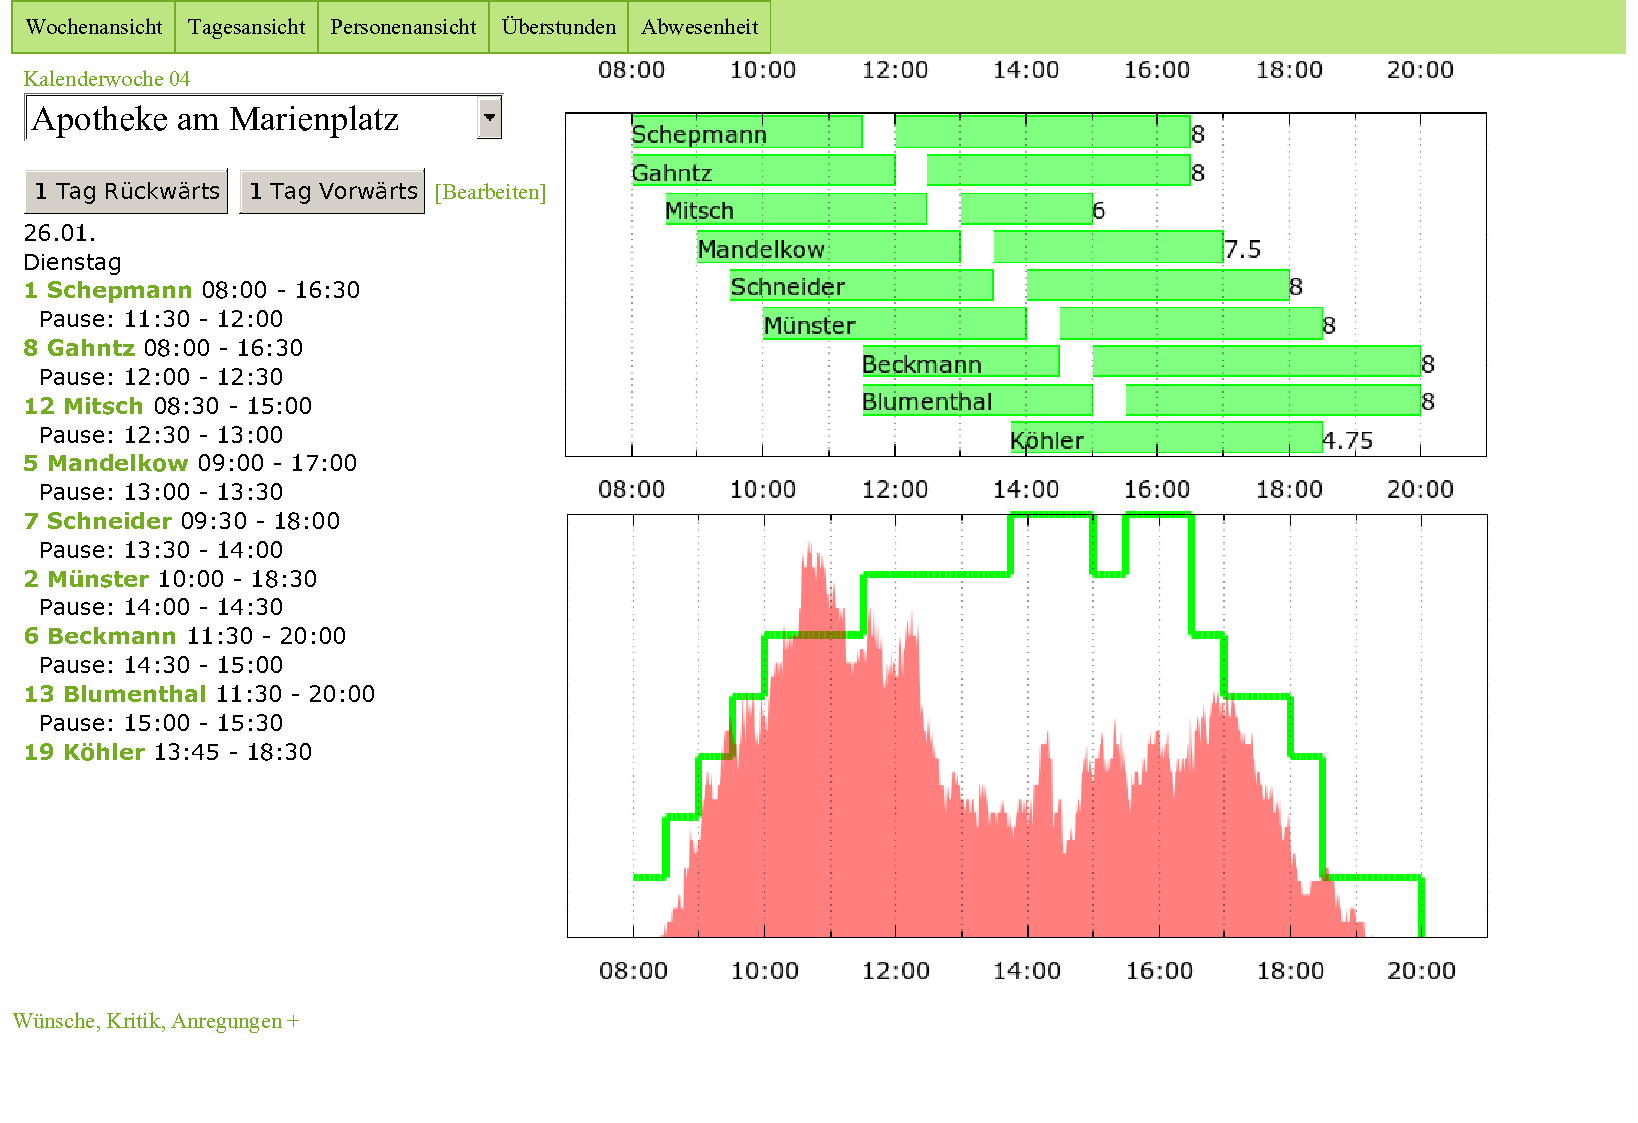
\includegraphics[width=0.8\textwidth]{tag-out}
\caption{Tagesansicht}
\label{fig:Tagesansicht}
\end{figure}

Als Navigationsmöglichkeiten sind lediglich die Schalter für einen Tag vor oder zurück gegeben. Es können alle Mandanten betrachtet werden.





\subsubsection{Woche}
Die Wochenansicht besteht aus einer Tabelle (Abb. \ref{fig:Wochenansicht}).
Für jeden Wochentag von Montag bis Freitag gibt es eine Spalte. In jeder Spalte sind die Mitarbeiter in der Reihenfolge des Dienstbeginns eingetragen.
\begin{figure}[h]
\centering
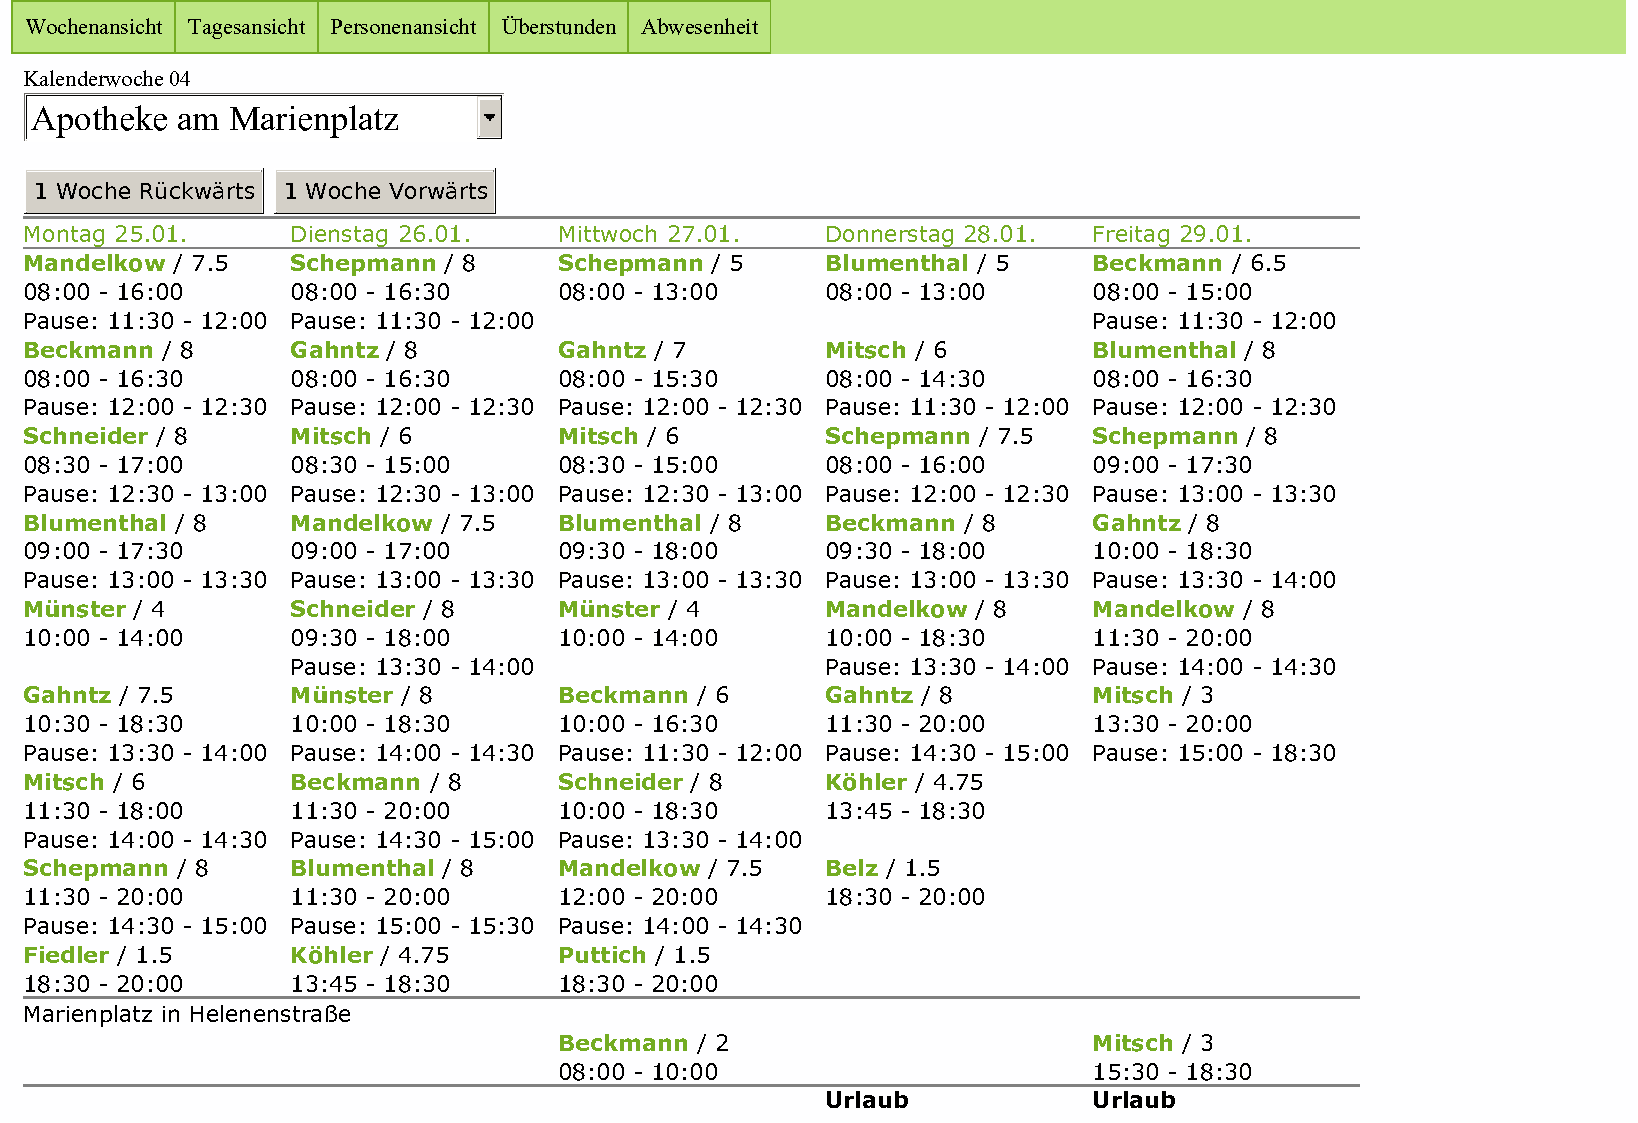
\includegraphics[width=0.8\textwidth]{woche-out}
\caption{Wochenansicht}
\label{fig:Wochenansicht}
\end{figure}

Unter dem ausgewählten Mandanten, wird auch eine zweite Tabelle angezeigt. Dort werden die Mitarbeiter gezeigt, die in den ausgewählten Mandanten gehören, aber in einer anderen Filiale eingesetzt werden.

Darunter werden die Mitarbeiter angezeigt die wegen Krankheit oder Urlaub nicht anwesend sind. Andere Abwesenheitsgründe (z.B. Elternzeit) werden nicht berücksichtigt.

Auch die Anzahl der Wochenstunden für jeden Mitarbeiter werden zusammengerechnet. Diese erscheinen nicht auf dem ausgehängten Ausdruck, da vor diesem Abschnitt ein Zeilenumbruch eingefügt wird.

Auch in dieser Ansicht kann jeweils eine Woche vor und zurück geblättert werden. Alle Mandanten können ausgewählt werden.





\subsubsection{Mitarbeiter}
In der Mitarbeiteransicht kann der Stundenplan eines einzelnen Mitarbeiters betrachtet werden.
In der Tabelle sind die Dienstzeiten der gesamten Woche von Montag bis Sonntag eingetragen.
Die Summe der Wochenstunden von Montag bis Freitag wird mit den Sollstunden verglichen. Abwesenheit durch Urlaub oder Krankheit werden von den Sollstunden automatisch abgezogen. Auch Feiertage werden beachtet.

Unter der Tabelle findet sich ein Bild, dass den Stundenplan graphisch darstellt (Abb. \ref{fig:Mitarbeiteransicht}).
\begin{figure}[h]
\centering
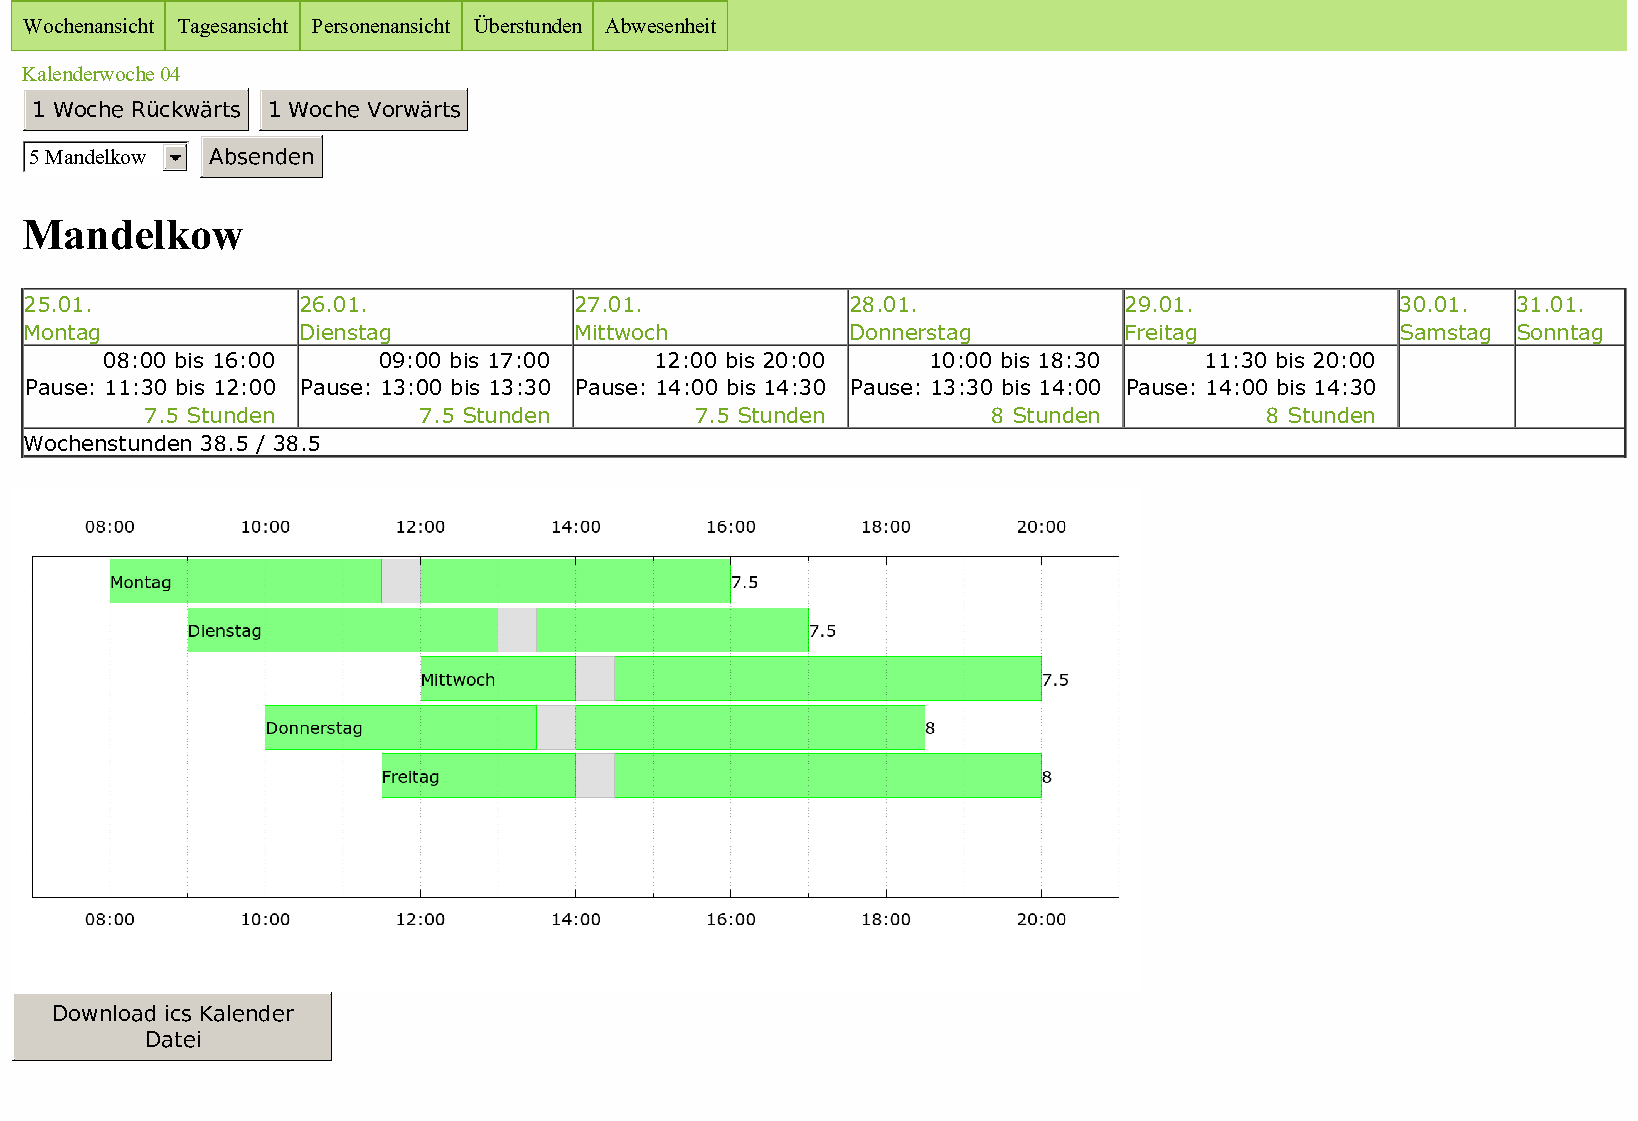
\includegraphics[width=0.8\textwidth]{mitarbeiter-out}
\caption{Mitarbeiteransicht}
\label{fig:Mitarbeiteransicht}
\end{figure}
Und darunter befindet sich ein Button, mit dem der Stundenplan als Kalenderdatei herunter geladen werden kann.



\paragraph{Technisches}
Die Datei hat das Format iCalendar (*.ics). Dies ist ein Datenformat zum Austausch von Kalenderinhalten. Es kann von den meisten gängigen Kalenderverwaltungsprogrammen (z.B. Google Kalender / Android Kalender, Microsoft Outlook, Blackberry Kalender Apps und iOS-Kalender) importiert werden.




\subsubsection{Stunden}
Die Überstunden werden in einer Tabelle für jeden Mitarbeiter angezeigt (Abb. \ref{fig:Stunden}).
Die Reihenfolge orientiert sich \emph{nicht} am Datum der Überstunden, sondern am Datum der Eintragung (unsichtbar). Das ist notwendig um das Saldo der Stunden korrekt zu addieren und zu subtrahieren.

\begin{figure}[h]
\centering
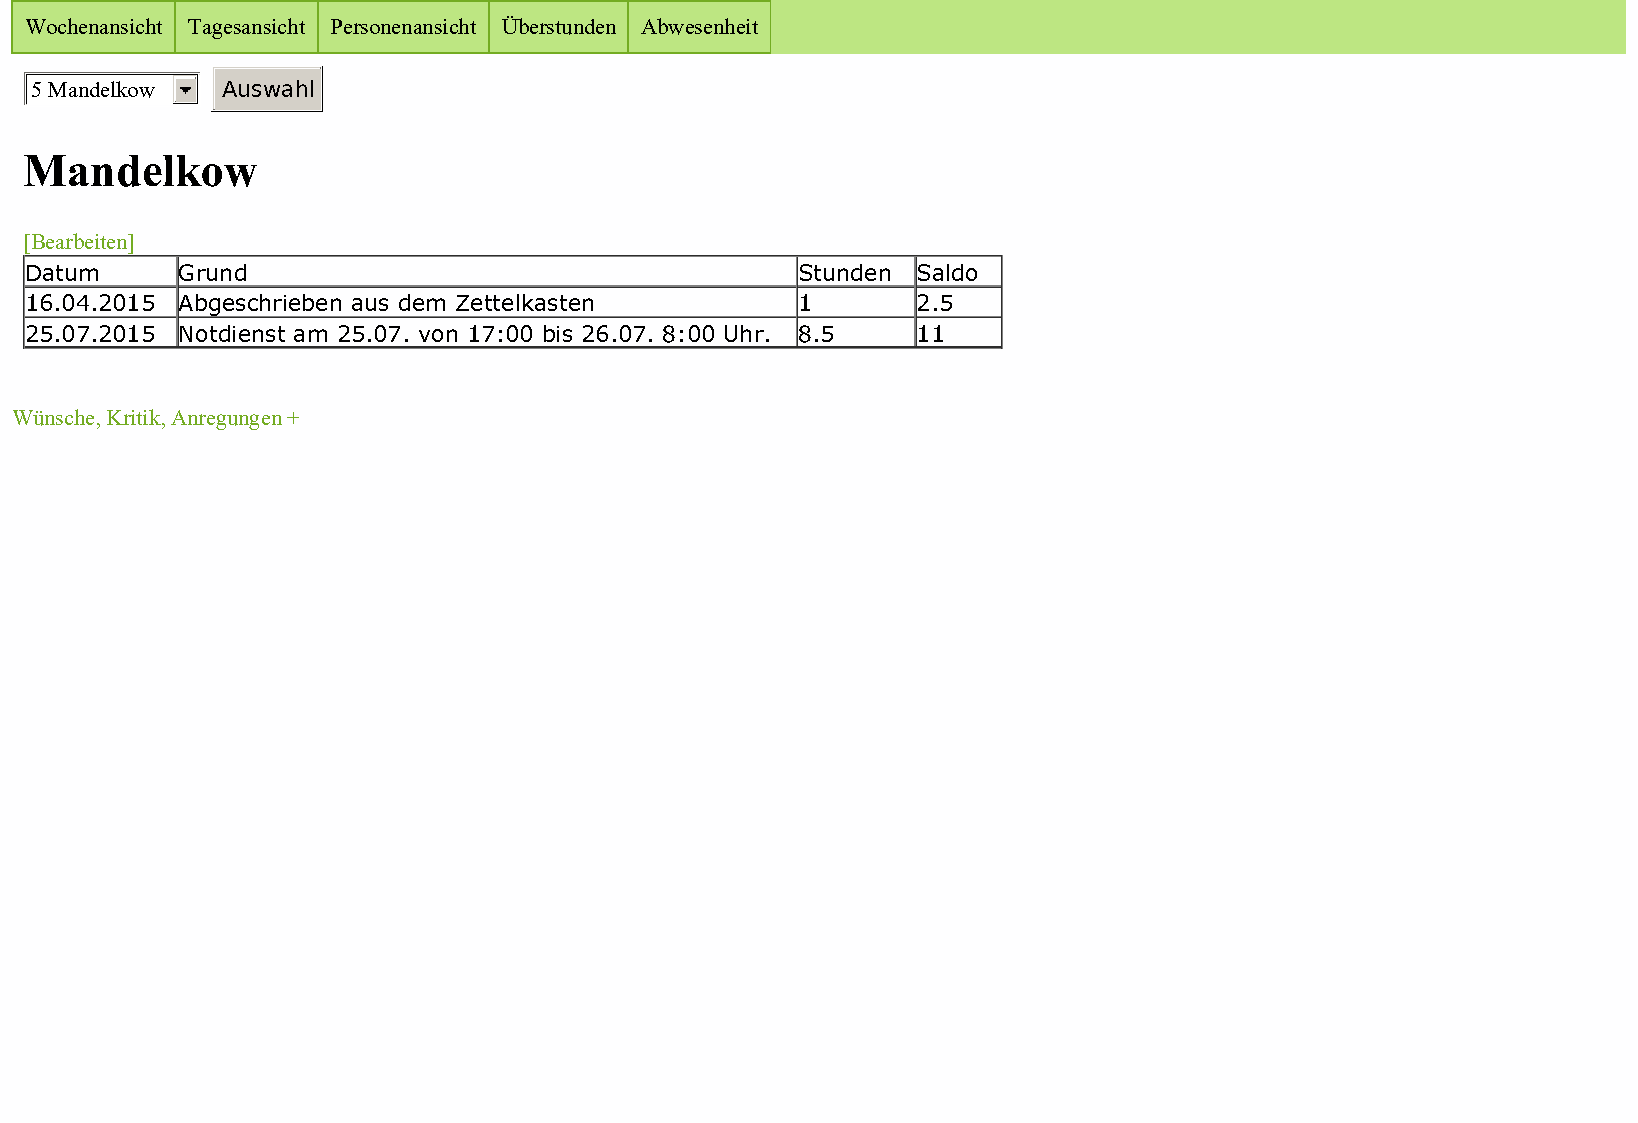
\includegraphics[width=0.8\textwidth]{stunden-out}
\caption{Stunden}
\label{fig:Stunden}
\end{figure}


\subsubsection{Abwesenheit}
Abwesenheitstage werden für jeden Mitarbeiter einzeln in einer Tabelle angezeigt (Abb. \ref{fig:Abwesenheit}).
Als Abwesenheit werden derzeit ausschließliche volle Tage gewertet. Es ist noch nicht möglich, einzutragen, dass jemand um 11 Uhr einen Zahnarzt-Termin hat und danach wieder zur Verfügung steht.

\begin{figure}[h]
\centering
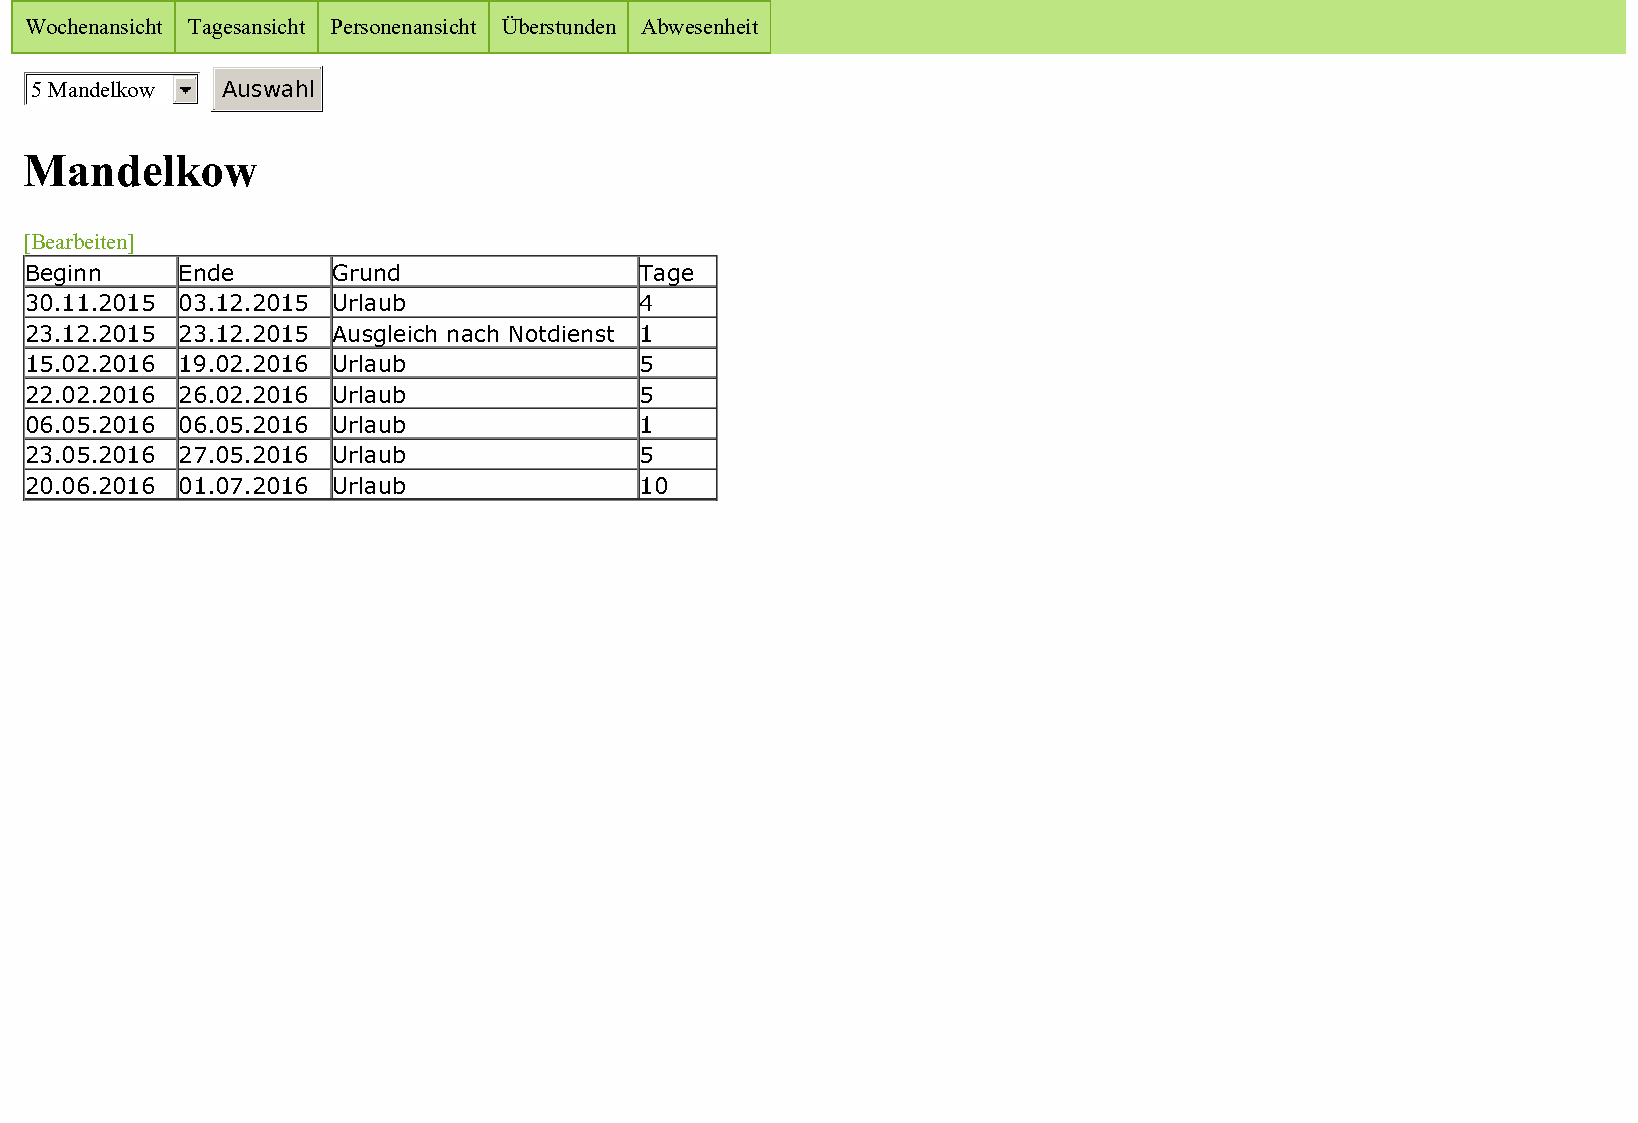
\includegraphics[width=0.8\textwidth]{abwesenheit-out}
\caption{Abwesenheit}
\label{fig:Abwesenheit}
\end{figure}

Zu den Gründen für Abwesenheit zählen neben Urlaub und Krankheit auch Elternzeit, Notdienst-Ausgleich oder Überstunden-Abbau.

An einem bestimmten Tag kann nur eine Abwesenheit pro Mitarbeiter starten. Allerdings wird noch nicht auf Überschneidungen geprüft.




\subsubsection{Offline}
Zu allen Informationen liegen auch offline Versionen in der Apotheke vor.
An der Pinnwand sollte der aktuelle Wochenplan und der Plan der folgenden Woche zu finden sein. Auch die Tagesansichten der aktuellen Woche inklusive Samstag werden dort ausgehängt. Über den Abholern befindet sich eine rote Box mit der Aufschrift "Arbeitszeitverschiebungen". In ihr werden Überstunden und deren Abbau eingeschrieben.
Hinten bei den Spinten hängt ein Jahresplan, auf dem die Urlaubszeiten eingetragen wurden.


\subsection{Eingabe zum Schreiben}
\subsubsection{Zugang}
Der Zugang zu den Eingabe-Masken liegt derzeit nur für Dr. Martin Mandelkow vor. Eine Vertretung sollte jedoch in Zukunft bestimmt werden.

\subsubsection{Tag}
\subsubsection{Woche}
\subsubsection{Mitarbeiter}
Es existiert keine Schreibversion der Mitarbeiter-Ansicht.
\subsubsection{Stunden}
\subsubsection{Abwesenheit}
Die Abwesenheitszeiten werden in dem roten Kästchen mit der Bezeichnung Arbeitszeitverschiebungen verwaltet. DOrt kann jedermann seine Überstunden eintragen. Jede Eintragung sollte durch einen Zweiten abgezeichnet werden (Vier-Augen-Prinzip).
\subsubsection{Upload}
Um die Daten des zu erwartenden Arbeitsaufwandes aktuell zu halten, sollte in regelmäßigen Abständen z.B. quartalsweise eine PEP-Datei in ASYS exportiert werden und zum Server hochgeladen werden.



\section{Systemvorraussetzungen}
	\begin{itemize}
		\item HTTP-Server (z.B. Apache)
		\item PHP 5.5
		\item MYSQL 4.1
		\item Gnuplot 5.0
	\end{itemize}










\section{To Do}
\begin{itemize}
	\item Eventuell eine PHP-Rechteverwaltung für Benutzer
	\item PHP-Interface für Mitarbeiterverwaltung (wird derzeit per phpmyadmin durchgeführt)
\end{itemize}










\end{document}
